\documentclass[12pt]{article}

\usepackage{a4wide}
\usepackage{graphicx}
\usepackage{url}
\title{Functional requirements of a generic tracking toolkit}
\author{Ch. Rosemann, DESY}
\date{\today}



\begin{document}
\maketitle 
\abstract{In order to be useful, a generic software toolkit has to meet several requirements of different types.
The tracking toolkit that is developed within the AIDA framework is no exception to this.
Generic requirements might include 'ease of use' or 'usability'.
A more formal description in these terms is already given in the project description.\\
This document is adressing the functional requirements, what kind of tasks the toolkit is to provide.
Its primary focus rests on the questions that the toolkit needs to provide an answer to.
The secondary focus is put on the specific algorithms which the toolkit can be interfaced to.
The purpose of this is primarily the design, both of its interface to the user, as well as the shape of the underlying design.  
}

\section{The background: a generic tracking toolkit}
These are the design requirements for the generic tracking toolkit, as defined in AIDA work package 2 -- common software tools, part 4.
Citing from~\cite{aida2.4}, the general design requirements are:
\begin{itemize}
    \item a well-defined modular approach
    \item a clearly defined API
    \item the separation of framework functionality, data and algorithmic content
    \item a flexible core framework
    \item a well-defined functionality for use in external reconstruction software
    \item allowing easy addition or extension of algorithms
    \item multi-core architecture foreseen in core framework
\end{itemize}
Without explicit statement, the close connection and interfacing with the generic geometry toolkit is assumed.
This is developed also in the context of work package 2 within the AIDA project.\\

The main purpose for using the tracking toolkit are track fitting and track finding.
While track fitting is in most parts a well established mathematical procedure, the usability for track finding needs to be defined in more detail.
By it's nature track finding depends very strongly on the type of experiment that is carried out, and the environment and requirements of it.
There are two general distinctions to be made: global and local track finding methods.
The tracking toolkit provides functionality to local track finding.
Characteristic of local track finding is the very tight coupling to the geometry.
Global methods usually don't rely on seeds and possibly take a geometry independent approach.

\section{General description}
There are two parts to the design.
The first layer is the part, with which a user interacts.
This will be briefly introduced, as it outlines the appearance to the outside.
The second part is the internal structure, which is needed to fulfill the functional requirements.\\
\subsection{Public API}
This consists of two main pieces, which are presented in figure~\ref{fig:mss}.
\begin{itemize}
    \item the master interface to the toolkit, allowing instantiation and configuration and
    \item the main trajectory class, which is main user API and has/hides the underlying algorithms.
\end{itemize}
The scheme of using only configured Tracjectory objects can be changed if needed.
\begin{figure}[h!]
 \begin{center}
 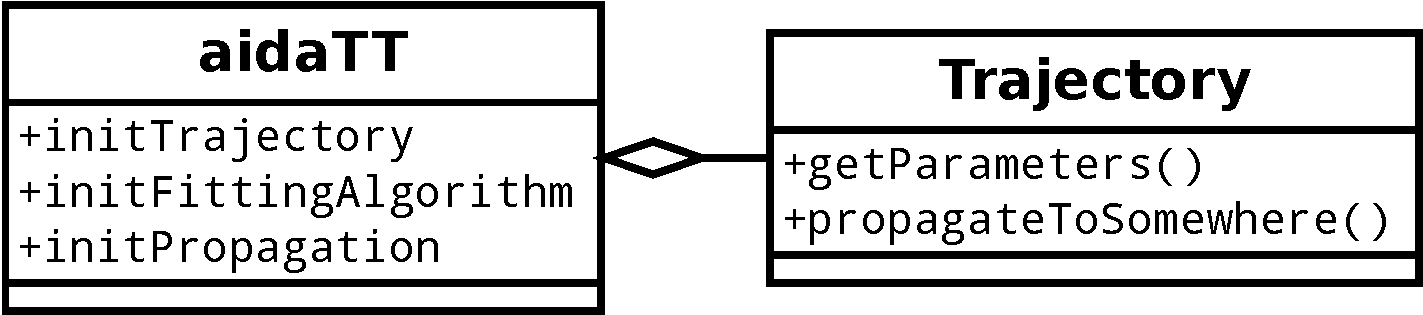
\includegraphics[width=.66\linewidth]{most_simple_structure.pdf}
 \end{center}
 \caption{The two main pieces of the tracking toolkit.}
 \label{fig:mss}
\end{figure}

 \subsection{An existing prototype for user interaction}

 \begin{minipage}{0.6\textwidth}%
 The central element for user interaction is the {\em Trajectory} class, created through the initialisation interface provided through the {\em aidaTT} class.
 The prototype, or basic design to build from is implemented in the {\em MarlinTrk} package.
 Therein, the system setup is done through the {\em IMarlinTrkSystem} class, by which an {\em IMarlinTrack} is created.
 The class structure is layed out with a Kalman Filter in mind; currently the only implementation is done for a Kalman Filter
 \\
 The same functionality is supposed to be provided as for the {\em MarlinTrack}.
 A simplified signature of this class is shown in the adjacent figure.%~\ref{fig:marlintrack}.
\end{minipage}%
\begin{minipage}{0.4\textwidth}%
 %\begin{center}%
 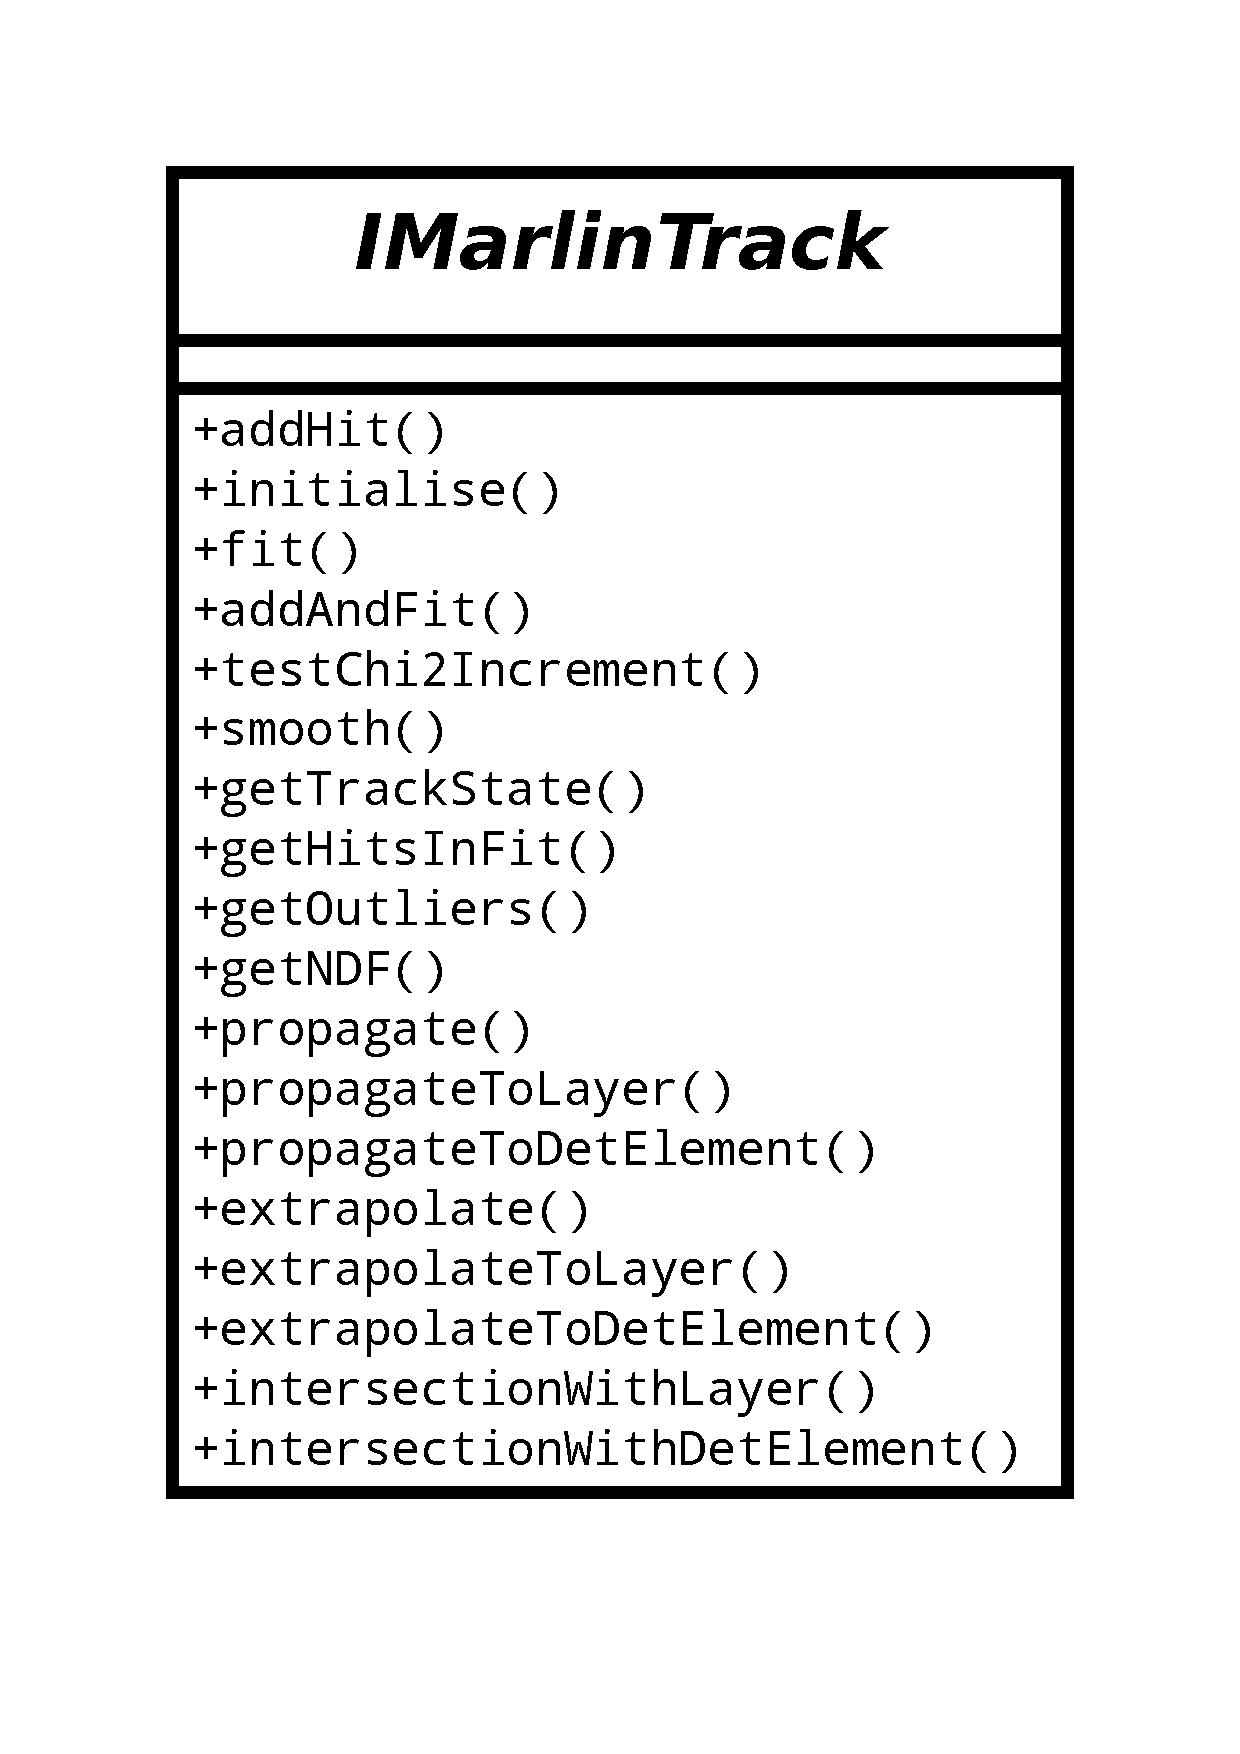
\includegraphics[width=.9\linewidth]{IMarlinTrk_simplified.pdf}%
 %\end{center}%
 %~ \caption{The simplified signature of IMarlinTrack, the ancestor class in idea to aidaTT::Trajectory.}%
 %~ \label{fig:marlintrack}%
\end{minipage}
   %~ \begin{figure}[h!]
 %~ \begin{center}
 %~ 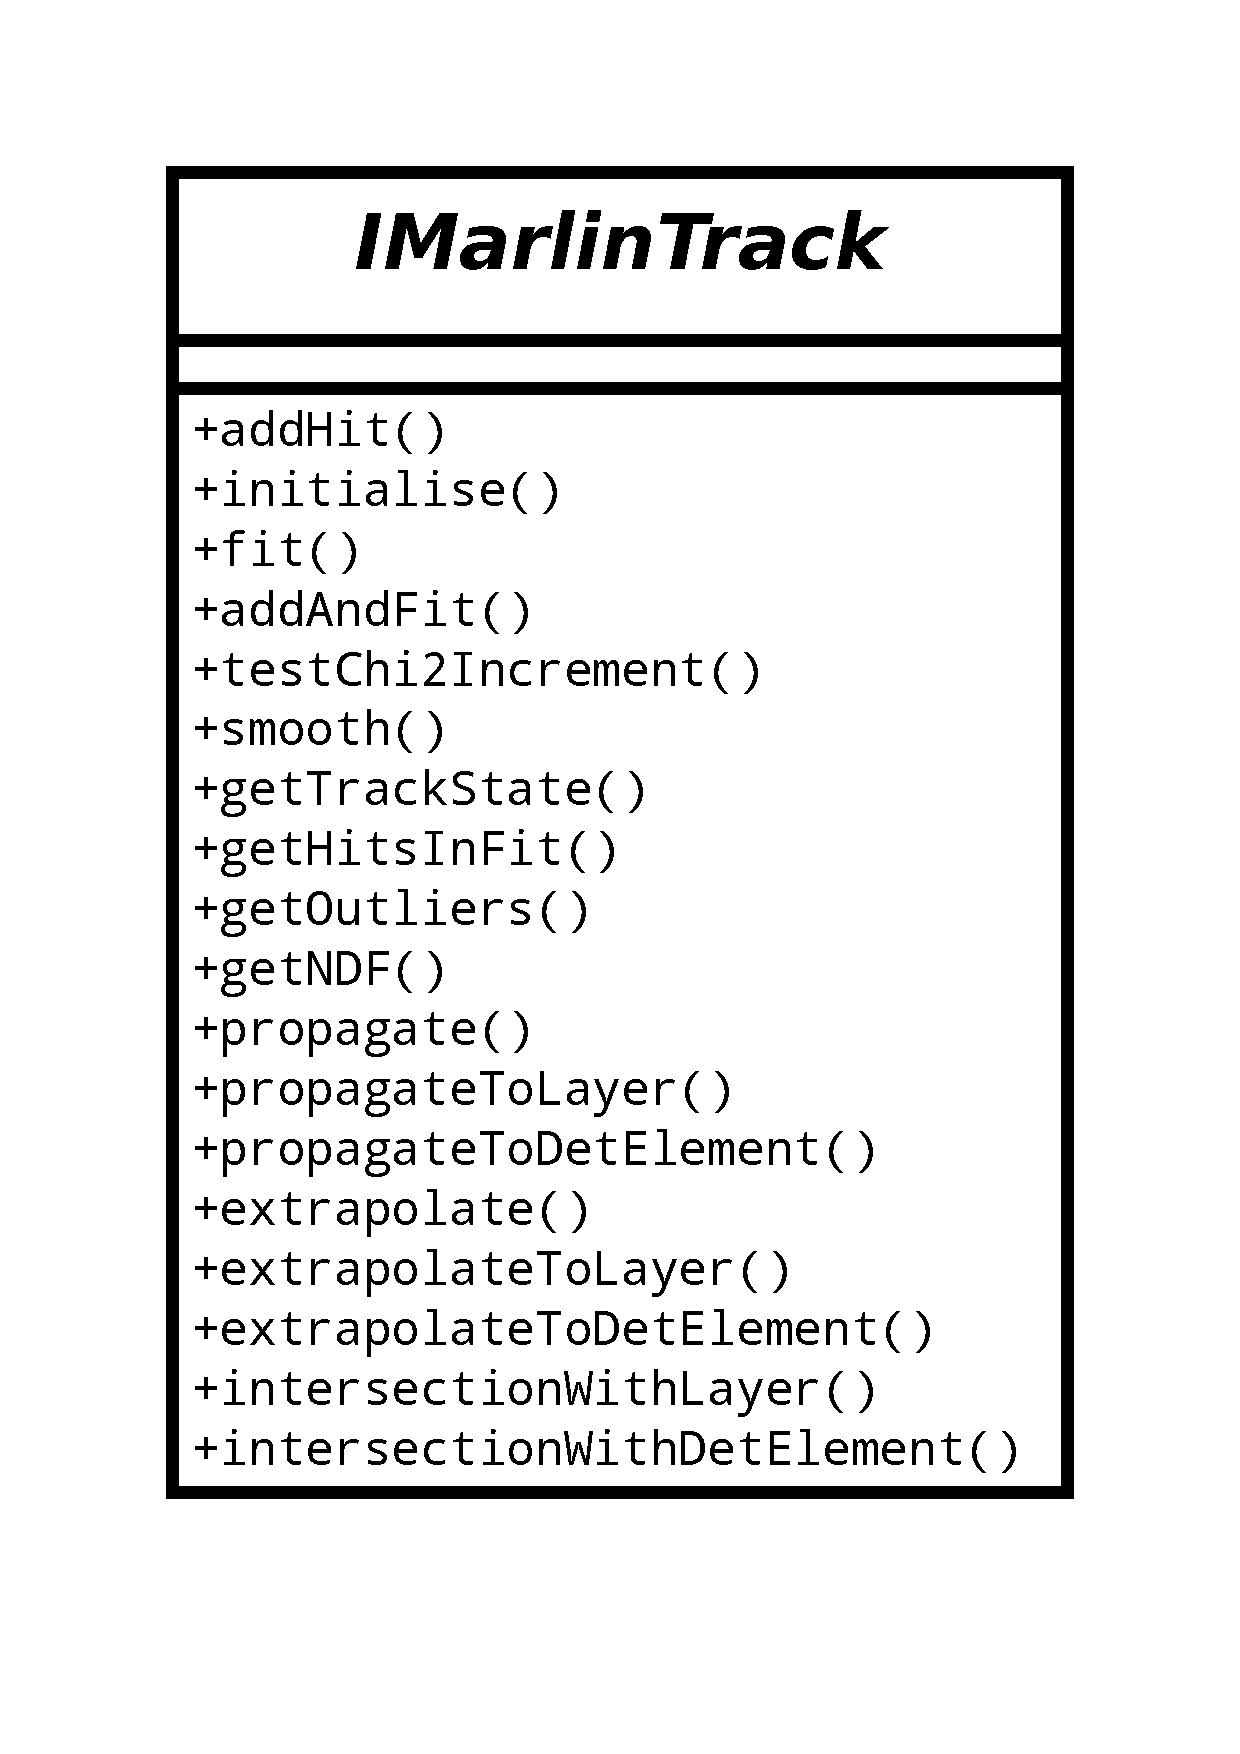
\includegraphics[width=.4\linewidth]{IMarlinTrk_simplified.pdf}
 %~ \end{center}
 %~ \caption{The simplified signature of IMarlinTrack, the ancestor class in idea to aidaTT::Trajectory.}
 %~ \label{fig:marlintrack}
 %~ \end{figure}


\subsection{Internal structure}
Internal to the toolkit is the representation of the different parts that allow manipulations of tracks, for example like parameter estimation (fitting), extrapolation/propagation and material interactions.
The definition of fitting algorithm is represented as an interface class.
Extrapolation and propagation ($\approx$ extrapolation including material effects) functionality is also provided with an interface class.
This first level of this extension is shown in figure~\ref{fig:bs}.
 \begin{figure}[h!]
 \begin{center}
 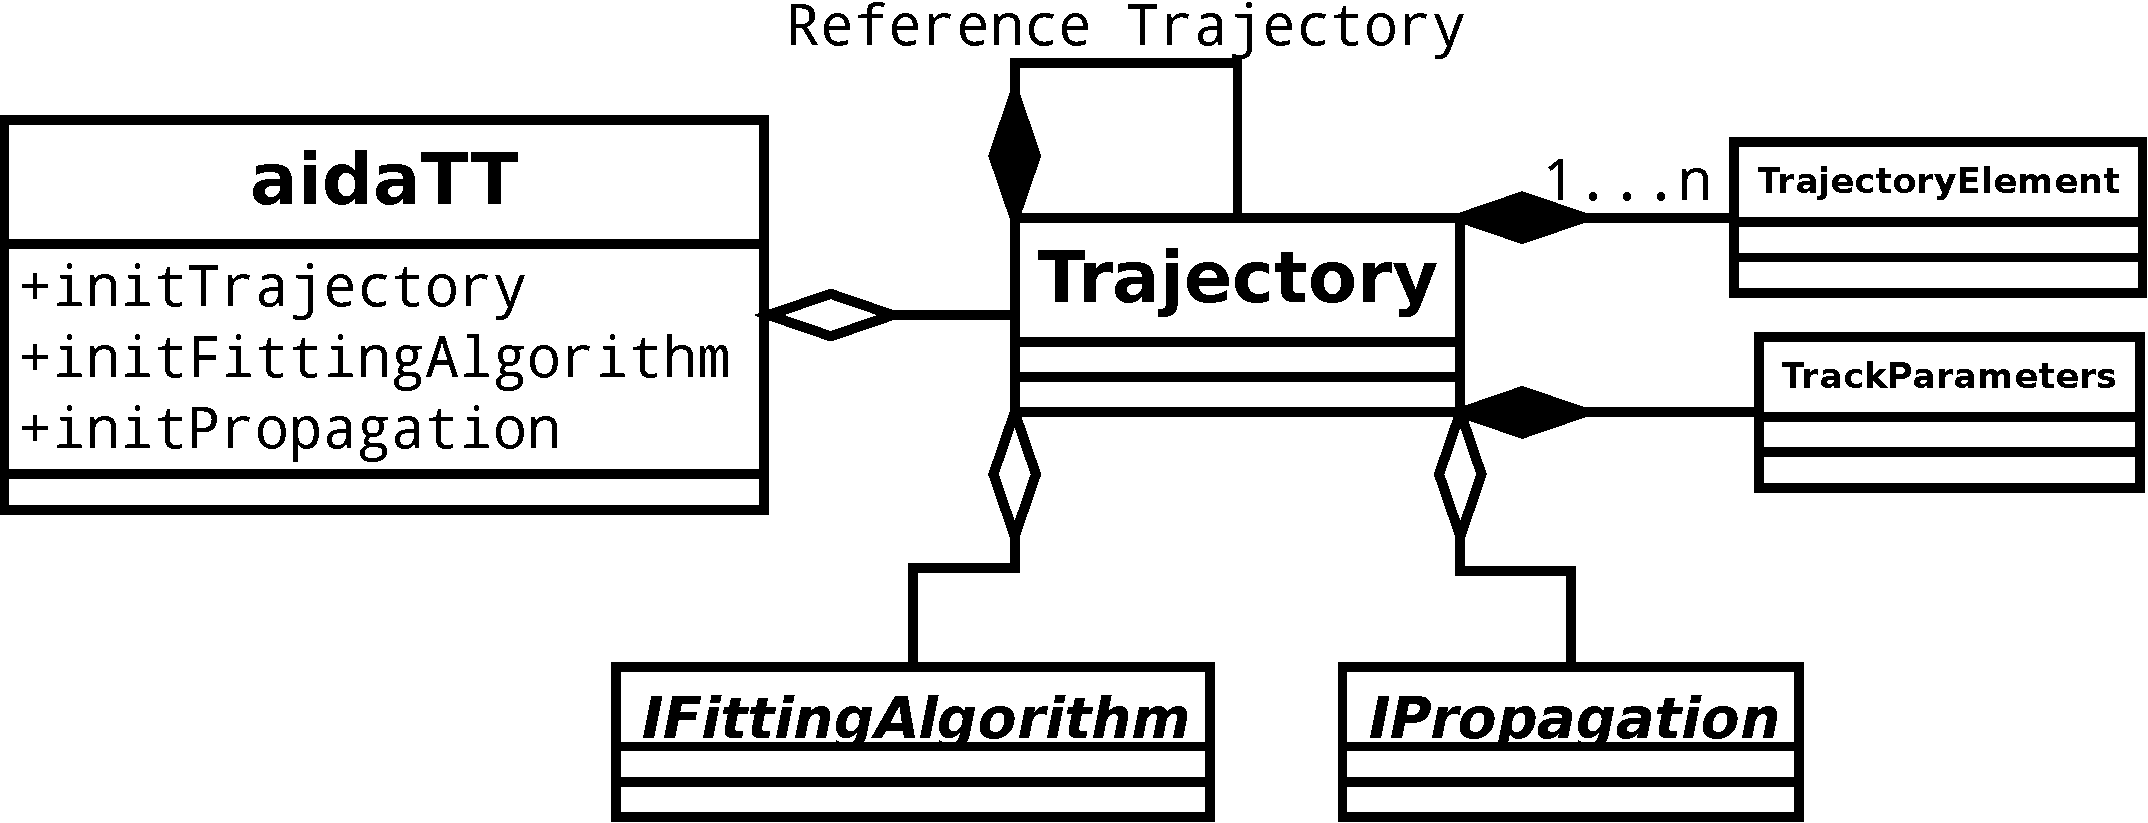
\includegraphics[width=.66\linewidth]{basic_structure.pdf}
 \end{center}
 \caption{The first level of extension to the aidaTT::trajectory class; which are the interfaces to the fitting algorithm and the propagation package.}
 \label{fig:bs}
 \end{figure}
 
The second extension completes the internal functionality by describing the {\bf trajectory elements} in more detail.
The trajectory elements themselves are an ordered list of {\em points} (for the lack of a better name) on the trajectory.
Anything directly associated to a trajectory can be identified uniquely and ordered by a real number: the arc length with respect to the chosen point of reference.
This basic layout is shown in figure~\ref{fig:teb}.
 \begin{figure}[h!]
 \begin{center}
 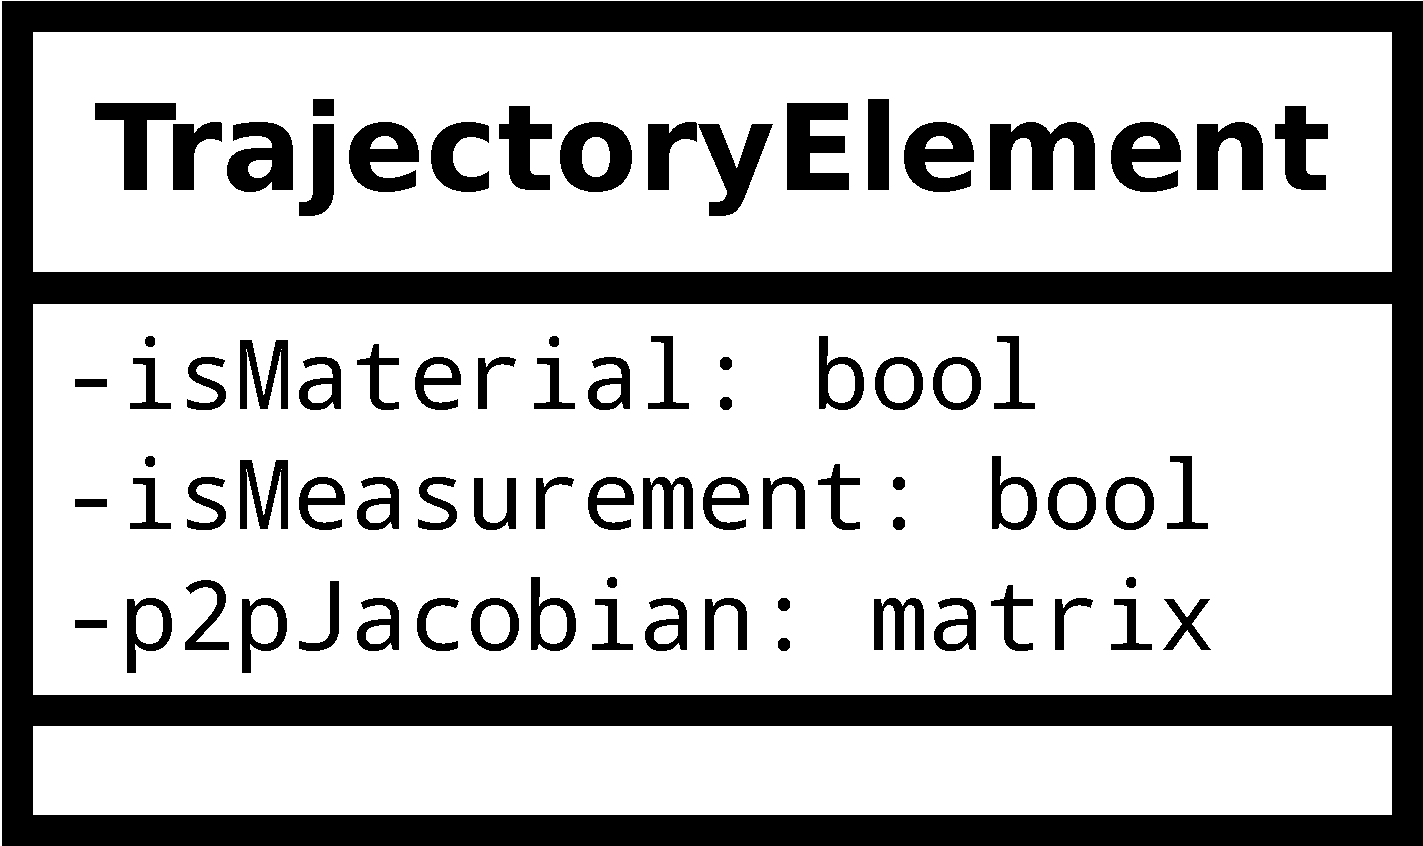
\includegraphics[width=.22\linewidth]{trajectory_element_simple.pdf}
 \end{center}
 \caption{The basic layout of a trajectory element: it is either material or a measurement -- or neither; plus the description to get to the next element.}
 \label{fig:teb}
 \end{figure}

Any element can further be categorized by being a non-exclusive member of the groups 
$$ \{\mathrm{Material}\} \otimes \{\mathrm{Measurement}\}.$$
Examples: 
\begin{itemize}
    \item an energy deposition on a silicon detector falls into both categories: scattering material and measurement;
    \item a signal on a wire in a wire chamber is only a measurement, but without material;
    \item the possible interaction with any kind of support material is no measurement;
    \item the estimation at any point without any material nor detector falls into neither category -- e.g. the values at the nominal interaction point.
\end{itemize}
In addition to the position of an individual element, the track is complete by the description of how to get from one {\em TrajectoryElement} to the next.
The material information, as well as the information about the orientation of measurement surfaces and the associated errors is directly connected to the geometry description.
The specific information about errors and orientation of measurement surfaces is encapsulated in an own abstract interface: {\bf IMeasurementSurface}.
This and the material information in {\bf IMaterial} is associated to an abstract geometry interface.
All this is shown in figure~\ref{fig:te}, which shows the basic design of the trajectory elements.
 \begin{figure}[h!]
 \begin{center}
 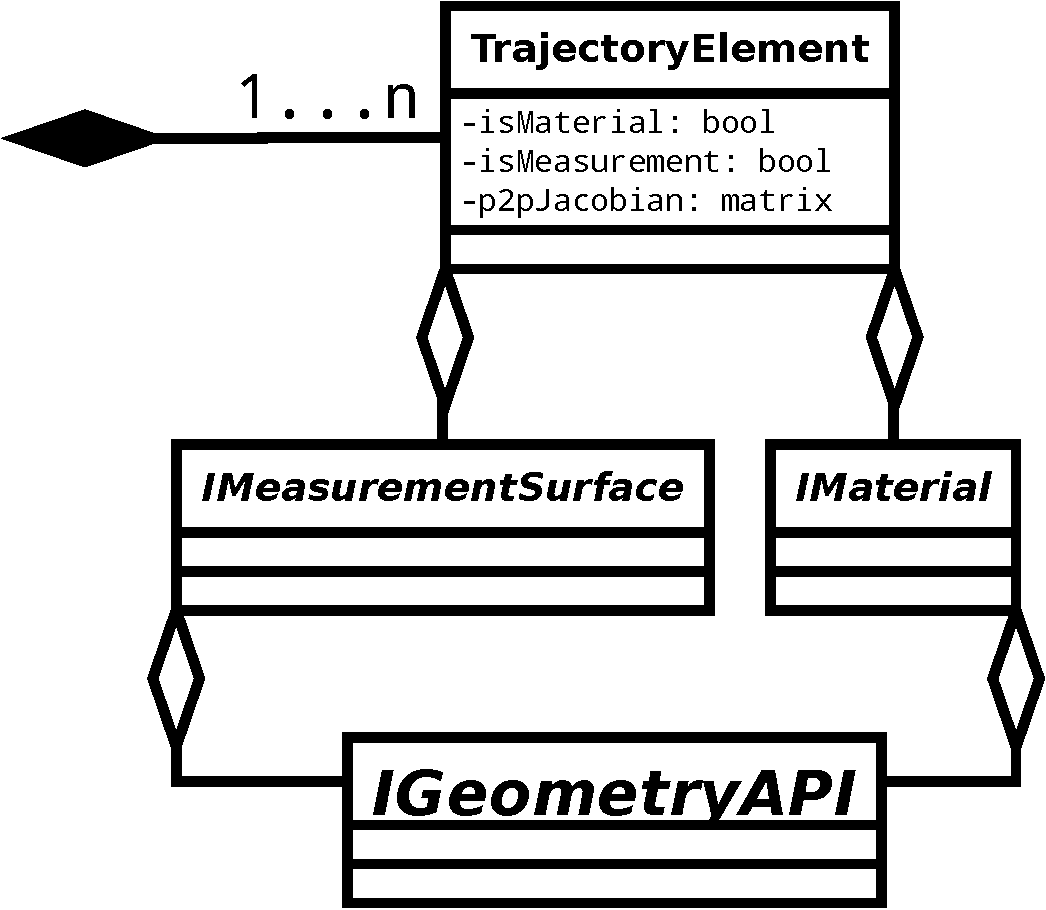
\includegraphics[width=.5\linewidth]{trajectory_element.pdf}
 \end{center}
 \caption{The second level of extension to the aidaTT::Trajectory class, focussing on the details of the trajectory elements.}
 \label{fig:te}
 \end{figure}

\subsubsection*{Measurements}
In parameter estimation the most important parts are the measurements, which constrain the trajectory.
Apart from being the basis for the estimation, measurements are special, since they are always uniquely connected to a detector.
For the description of a measurement the following components are needed:
\begin{itemize}
	\item the measurement surface and the coordinates on that surface\\
		this can be either global or local -- both can be accessed via the geometry
	\item the measurement directions of the detector, $\vec{u},\vec{v}$
	\item the uncertainty of the measurement
\end{itemize}
There are different concepts, how this information is passed/accessible.
Measurements are most often defined by global coordinates and the (equally global) covariance.
The surfaces (in terms of  $\vec{u},\vec{v}$) can be included, but usually this is accessed indirectly by using geometry functionality.

In principle either combination of objects and information access is possible.
Chosen (for now) is the model that a measurement contributing to a trajctory in aidaTT is:
\begin{itemize}
	\item a global coordinate,
	\item a reference (e.g. pointer) to the measurement surface in the geometry (which contains the local measurement directions)
	\item the uncertainties w.r.t. the measurement directions.
\end{itemize}
	

\subsection{The overall structure}
The complete structure, without most implementation details is depicted in figure~\ref{fig:total}.
 \begin{figure}[h!]
 \begin{center}
 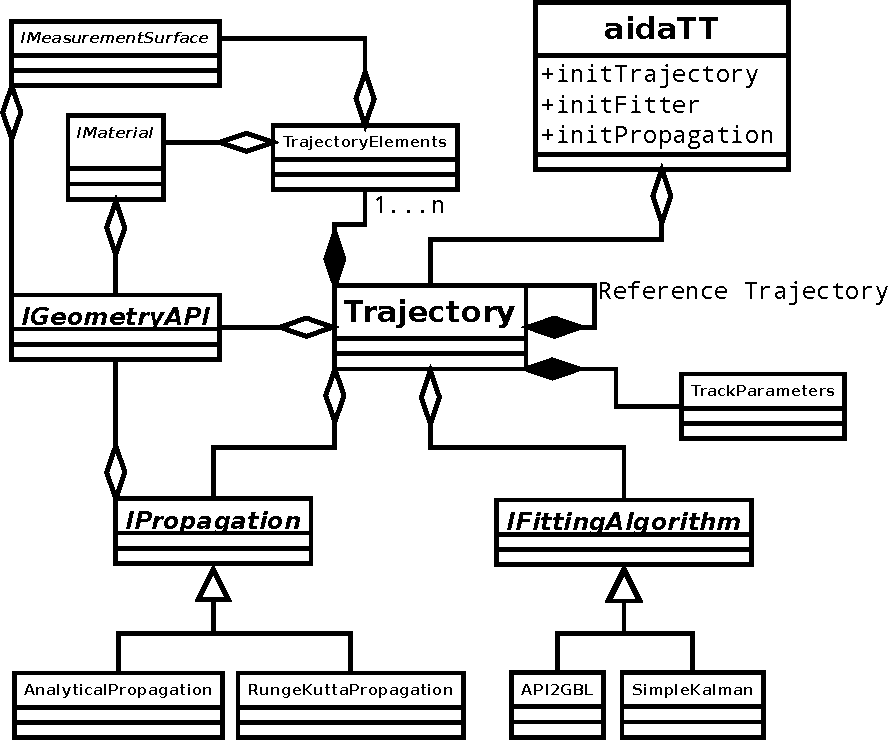
\includegraphics[width=\linewidth]{overall.pdf}
 \end{center}
 \caption{The complete layout of the generic tracking toolkit.
 The core parts are visible, as well as ideas for specific implementation about the two abstract interfaces.
 For the fitting algorithms these are the GeneralBrokenLines~\cite{GBL} and a Kalman Filter.
 For the propagation these are the numerical solution or an analytical one.}
 \label{fig:total}
 \end{figure}
 
\newpage

%%%%%%%%%%%%%%%%%%%%%%%%%%%%%%%%%%%%%%%%%%%%%%%%%%%%%%%%%%%%%%%%%%%%%%%%%%%%%%%%
%%%%%%%%%%%%%%%%%%%%%%%%%%%%%%%%%%%%%%%%%%%%%%%%%%%%%%%%%%%%%%%%%%%%%%%%%%%%%%%%


\section{Assumptions}
There are several limitations built in, some of them are implicit.
This is a first, short list on the most obvious ones:

\subsection{Track parameter representation}
The parametrization of the track is the (local) curvilinear system.
The great advantage is, that for this system the complete analytical description for any kind of propagation exists.
This is most important for the propagation of covariances, as described in~\cite{strandlie}.\\
Furthermore, for this track representation a numerical solution of the initial value problem exists as a routine.
The original formulation is in FORTRAN~\cite{geane}, but a new implementation in C++ is available in~\cite{genfit}.\\
The track representation is also important, since the projected crossing point to a measurement surface needs to be calculated.
There are two choices: either let the user specify the projection (matrix) from track system to measurement.
Or fix the choice of system to be able to code the calculation.

\subsection{All trajectory elements must be ordered in arc length}
Prior to instantiation of the trajectory, all elements {\bf must} be ordered in arc length.

\subsection{Provision of all elements of interest at instantiation time}
All elements (measurements, material, {\em hits} and points of interest) must be provided during the initialization of the trajectory.

\subsection{Provision of Point to Point Transport}
It is assumed that for track parameter estimation ({\em track fitting}) a reference trajectory is known.
Following this reference trajectory, every transport matrix is known -- at least in principle.
The user can specify this during initialization, or use the propagation methods to synthesize this matrices.

\subsection{Use for track finding}
There have been tries to generalize pattern recognition algorithms, and to create toolkits to perform the task.
In general, every detector design with a specific environment faces different challenges.
Some methods require knowledge of the detector layout, e.g. individual errors of different detector elements, or their positions.
\\
In principle the use with a pattern recognition algorithm is possible; it still remains to be seen if it's worthwile to implement special functionality towards that end.


%%%%%%%%%%%%%%%%%%%%%%%%%%%%%%%%%%%%%%%%%%%%%%%%%%%%%%%%%%%%%%%%%%%%%%%%%%%%%%%%
%%%%%%%%%%%%%%%%%%%%%%%%%%%%%%%%%%%%%%%%%%%%%%%%%%%%%%%%%%%%%%%%%%%%%%%%%%%%%%%%


\section{Interfaces and pseudo-code snippets}
All classes share a single namespace called "aidaTT".
This is implicit in all the given pseudocode snippets, and made explicit only in the headings.
The interfaces between the classes can be divided into the internal and external parts.
Internal are the ones that connect the different classes within the aidaTT.
External ones are either exposed to an user, the outside world or external parts of the framework.

\subsection{Master class: aidaTT::aidaTT}
aidaTT is the main interaction class to instantiate a trajectory, and to configure the different components.
Depending on the needed functionality, the following parts have to be initialized:
\begin{itemize}
    \item Either of the following two options
        \begin{itemize}
            \item the elements of a trajectory: \\at least a collection of measurements\\ if no propagators are given, they are synthesized as needed
            \item an existing trajectory
        \end{itemize}
    \item the fitting algorithm; which imposes the provision of additional information specific to the chosen type
    \item the method of propagation; which also takes different additional arguments
    \item the entry point to the geometry, which fulfills the interface definition
\end{itemize}
Any further interaction then happens with the returned {\tt trajectory}.

\subsubsection{Pseudo-code snippets for aidaTT::aidaTT}

\subsection{User interface to aidaTT::Trajectory}
The use of a {\tt trajectory} can range from simply storing a collection of measurements along with an estimation of the associated track parameters, up to the full information about the trajectory.
This includes all materials that are crossed, parameters and their uncertainty at each element.
The 

\subsubsection{Pseudo-code snippets for aidaTT::Trajectory}


%\subsection{Algorithmic interface to aidaTT::trajectory}


%%%%%%%%%%%%%%%%%%%%%%%%%%%%%%%%%%%%%%%%%%%%%%%%%%%%%%%%%%%%%%%%%%%%%%%%%%%%%%%%
%%%%%%%%%%%%%%%%%%%%%%%%%%%%%%%%%%%%%%%%%%%%%%%%%%%%%%%%%%%%%%%%%%%%%%%%%%%%%%%%


\section{Open questions}
\begin{itemize}
    \item Optional running of more than one fitting algorithm?\\
		No, this doesn't make much sense. Every track is tightly coupled to the fitter that was used.
    \item Optional running of more than one propagation method?\\
		No, also doesn't make much sense. This can probably be done ''as needed''.
    \item Only one geometry interface!
\end{itemize}

\section{Implementation strategy}
Natural guideline: MarlinTrkSystem and MarlinTrack
\begin{enumerate}
    \item basic class layout with Python
    \item simple extensions: 
        \begin{enumerate}
            \item simple propagation possible
            \item fitter available
            \item fake geometry information
        \end{enumerate}
    \item python interface to TGeo?
    \item review interaction
\end{enumerate}


%%%%%%%%%%%%%%%%%%%%%%%%%%%%%%%%%%%%%%%%%%%%%%%%%%%%%%%%%%%%%%%%%%%%%%%%%%%%%%%%
%%%%%%%%%%%%%%%%%%%%%%%%%%%%%%%%%%%%%%%%%%%%%%%%%%%%%%%%%%%%%%%%%%%%%%%%%%%%%%%%


\begin{thebibliography}{99}
\bibitem{aida2.4} \url{http://cds.cern.ch/search?p=AIDA-D2.4}

\bibitem{GBL} C. Kleinwort. General Broken Lines as advanced track fitting method. NIM A673 (2012) 107-110.

%\bibitem{MarlinTPC} MarlinTPC Homepage: https://znwiki3.ifh.de/MarlinTPC/

%\bibitem{millepede} V. Blobel. Software Alignment for Tracking Detectors. NIM A566 (2006) 5-13.

%\bibitem{l3helix}  J. Alcaraz. Helicoidal tracks. L3 Internal Note 1666 (1995)

\bibitem{strandlie}  A. Strandlie, W. Wittek. Derivation of Jacobians for the propagation of covariance matrices of track parameters in homogeneous magnetic fields. NIM A566 (2006), 687-698

\bibitem{geane} M.Innocente,V.Mairie,E.Nagy,GEANE: Average tracking and error propagation package, CERN Program Library,W5013-E,1991.

\bibitem{genfit} C.H\"oppner, S. Neubert, B. Ketzer, S. Paul. A novel generic framework for track fitting in complex detector systems. NIM A620 (2010), 518-525

\end{thebibliography}



\end{document}
